% L1a course-orientation deck.
%
% THIS DECK IS THE SOLE ARTIFACT FOR L1a AND IS AUTHORITATIVE ON ITS OWN.
%
% Every other lecture in the course mirrors a notebook or a notes packet, and
% every other deck header says so. L1a has neither, and that is deliberate:
%
%   - No notebook. The manifest records that none is required. The two
%     numerical preview figures are generated reproducibly by the figure build,
%     but students are not asked to compute in L1a.
%   - No notes packet. lectures/week-1/L1a/docs was deleted on 2026-08-19.
%     The notes were stale and substantially duplicative of the L1b deck, which
%     already teaches the policy-rate versus valuation-rate distinction two days
%     later. Recoverable from git history if anyone wants it back.
%
% DO NOT "fix" this asymmetry by regenerating notes from these slides. The
% asymmetry is the design. Because the deck is the only record, every slide has
% to be legible after the room empties: the promise table, the validation
% ladder, and the four reading links all carry their own statement of the point
% rather than leaning on a lecturer.
%
% Design spec: private/specs/2026-08-19-l1a-course-intro-redesign.md
%
% Frame order and the minute budget it serves (75 min total):
%
%   title                                     -> \vntitlepage
%   Disclaimer and Risks                      -> always second, house convention
%   Objectives for Today                      -> three objectives, house format
%   How This Course Runs                      -> logistics      20 min
%   How We Will Work                          -> logistics
%   Markets Connect Investors and Companies    -> future relevance  8 min
%   Market Scale Compared to Two Industries   -> market scale    6 min
%   Price Paid Versus Value Controlled        -> market scale
%   The Four Units of the Course              -> roadmap
%   Optimization Finds the Best...            -> numerical preview  3 min
%   Options Can Reshape...                    -> numerical preview  3 min
%   Every Unit Builds Toward the Same Decision -> decision      10 min
%   Each Test Exposes a New Way an Idea Can Fail -> decision
%   Five Promises for $10,000                 -> table + vote    5 min
%   What the Five Promises Are Called         -> reveal          3 min
%   Three Questions We Cannot Answer Yet      -> reveal
%   A Bank Failure in March 2023              -> SVB clip        7 min
%   Summary                                   -> three takeaways
%   Further Reading                           -> offered, not assigned
%
% No \transitionframe: that belongs to a concept-review opening, and this deck
% has none.
%
% The course map names "Treasury securities" early because that is the precise
% scope of Unit 1. The five specific promise names -- bill, note, bond,
% corporate bond, and TIPS -- still wait for "What the Five Promises Are Called".
\documentclass[aspectratio=169,11pt]{beamer}
\usepackage{vnslides}

% Course hub: syllabus, schedule, released materials, and setup instructions.
\newcommand{\policyurl}{https://github.com/varnerlab/CHEME-5660-CourseRepository-Fall-2026}

% PBS NewsHour, 28 March 2023, Paul Solman: "The factors behind Silicon Valley
% Bank's collapse." Runtime 6m04s, verified 2026-08-19, PBS-owned URL, no login.
% The segment explains that the bank bought government securities, rates rose,
% and it had to sell at a loss -- which is the answer to this deck's closing
% question. Play it in full and do NOT paraphrase it afterwards.
\newcommand{\svburl}{https://www.pbs.org/newshour/show/the-factors-behind-silicon-valley-banks-collapse}

\title{{\vnheavy L1a}: Course Orientation, Markets, and Financial Decisions}
\subtitle{CHEME 5660 Cornell University}
\author{Copyright Jeffrey Varner 2026. All Rights Reserved}

\begin{document}

% ---- title ---------------------------------------------------
\vntitlepage

% ---- disclaimer ----------------------------------------------
\begin{frame}{Disclaimer and Risks}
  \vspace{0.6em}
  \textbf{\ink{Training only.}} This content is for training and informational
  purposes only. The teaching team does not make, give, or endorse any offer or
  solicitation to buy or sell securities or derivative products, or provide
  investment or trading advice or strategy.

  \vspace{1.1em}
  \textbf{\ink{Risk.}} Trading involves risk and is generally not recommended for
  those with limited resources, experience, or a low risk tolerance. Past
  performance does not guarantee future success.

  \vspace{1.1em}
  \textbf{\ink{Responsibility.}} You are responsible for your investment decisions
  based on your financial circumstances, objectives, risk tolerance, and
  liquidity needs.
\end{frame}

% ---- objectives ----------------------------------------------
\begin{frame}{Objectives for Today}
  \vspace{0.4em}
  Today we answer how this course works, why financial
  markets matter even if you never become a trader, and what makes one investment
  preferable to another.

  \vspace{0.9em}
  \decklabel{Today's concepts}
  \vspace{0.4em}
  \begin{itemize}\setlength{\itemsep}{0.5em}
    \item \hilite{Course roadmap}: we'll explore three asset classes and combine them into strategies,
      making and testing financial decisions.
    \item \hilite{Why markets matter}: financial markets have societal impact. Most adults and Cornell itself are
      investors, while companies use public markets to raise money which funds the development of new products and services.
    \item \hilite{Our first decision problem}: today, we'll introduce our first decision problem. Investments pay different
      amounts at different times. How can we compare them?
  \end{itemize}
  \vspace{-0.4em}

  % \slidenote{Note:}{this lecture has no notebooks. These slides are the record.}
\end{frame}

% ==== logistics ====
\begin{frame}{How This Course Runs}
  \vspace{0.2em}
  Across twenty-eight lectures, we'll move from understanding financial assets to
  valuing them, combining them into portfolios, and making investment decisions.

  \vspace{0.65em}
  \begin{columns}[T,onlytextwidth]
    \begin{column}{0.305\textwidth}
      \eyebrow{Materials}
      \vspace{0.25em}
      {\small Download each week's materials from the repository Releases page, or clone
      the repository. Released files stay frozen; corrections are announced.}
    \end{column}
    \begin{column}{0.305\textwidth}
      \eyebrow{Tools}
      \vspace{0.25em}
      {\small Use Julia 1.12 through juliaup, Anaconda for Jupyter, and VS Code
      with the Julia extension. See the README for details.}
    \end{column}
    \begin{column}{0.305\textwidth}
      \eyebrow{Questions}
      \vspace{0.25em}
      {\small Ask questions on Ed Discussion rather than by email, so each answer
      reaches everyone with the same question.}
    \end{column}
  \end{columns}

  \vspace{0.8em}
  {\large\vnmedium\ink{Final project:}} automated trading with live data and live
  market access through the
  \href{https://alpaca.markets/}{Alpaca Markets application programming interface}.

  \slidenote{Policies:}{\href{\policyurl}{grading, attendance, academic integrity, and accommodations are posted in full}}
\end{frame}

% JDV doesn't want this frame in the deck, what is the point of it?
% It is a generic statement about the scientific method, not a course-specific point.
% The course map and the decision loop already show the same idea in a more specific way.
% \begin{frame}{Ask a Question, Build a Model, Test It}
%   \vspace{0.3em}
%   The same cycle appears in every unit.

%   \vspace{0.6em}
%   \begin{itemize}\setlength{\itemsep}{0.55em}
%     \item \hilite{Start with a question.} New concepts appear when they help us
%       solve a financial problem.
%     \item \hilite{Use code to explore.} Most code is provided; you will change
%       assumptions, inspect the results, and explain what the model does.
%     \item \hilite{Test against evidence.} A mathematically correct model can
%       still fail when its assumptions do not match reality.
%   \end{itemize}

%   \vspace{0.7em}
%   The goal is not just to get an answer. It is to know when that answer deserves
%   trust.
% \end{frame}

% ==== two-sided relevance ====
\begin{frame}{Markets Connect You, Cornell, and Companies}
  \vspace{0.1em}
  \begin{columns}[T,onlytextwidth]
    \begin{column}{0.285\textwidth}
      \eyebrow{Your side (2025)}

      \vspace{0.05em}
      {\fontsize{32}{34}\selectfont\vnmedium\hilite{61\%}\par}
      \vspace{0.05em}
      {\small of U.S. adults had a retirement account.}

      \vspace{0.3em}
      {\small How the account is invested determines the risk-reward trade-off.}

      \vspace{0.25em}
      {\small\dimmed{I'm a student, I don't have a retirement account yet.}}
    \end{column}
    \begin{column}{0.025\textwidth}
      \centering
      \vspace{0.05em}
      {\color{vnrule}\rule{0.5pt}{3.6cm}}
    \end{column}
    \begin{column}{0.32\textwidth}
      \eyebrow{Cornell's side (2025)}

      \vspace{0.05em}
      {\fontsize{32}{34}\selectfont\vnmedium\hilite{\$10.9B}\par}
      {\small FY2025 endowment}

      \vspace{0.3em}
      {\large\textbf{\hilite{\$498M}}}{\small\ 
      mainly from the endowment payout went to operations.}

      \vspace{0.3em}
      {\small About \hilite{29\% (\$3.16B)} of Cornell's endowment supported
      financial aid.}
    \end{column}
    \begin{column}{0.025\textwidth}
      \centering
      \vspace{0.05em}
      {\color{vnrule}\rule{0.5pt}{3.6cm}}
    \end{column}
    \begin{column}{0.31\textwidth}
      \eyebrow{Company side}

      \vspace{0.05em}
      {\fontsize{32}{34}\selectfont\vnmedium\hilite{315}\par}
      {\footnotesize corporate IPOs in U.S. markets}\par
      {\footnotesize 01/2025 - 06/2026}

      \vspace{0.2em}
      {\footnotesize An IPO lists a private company's shares on a public market.}

      \vspace{0.2em}
      {\footnotesize\textbf{\hilite{Raise capital}} by selling new shares;
      \textbf{\hilite{create liquidity}} by letting shareholders trade.}
    \end{column}
  \end{columns}

  \slidenote{Sources:}{\href{https://www.federalreserve.gov/publications/2026-economic-well-being-of-us-households-in-2025-savings-investments.htm}{Fed SHED, 2025}; \href{https://finance.cornell.edu/sites/default/files/cornell-financial-report-FY2025.pdf}{Cornell FY2025 report}; \href{https://finance.cornell.edu/financial-guide/statement-activities}{Cornell activities}; \href{https://www.sec.gov/data-research/statistics-data-visualizations/initial-public-offerings-ipos}{SEC IPO data}}
\end{frame}

% ==== engineer ====
% TWO frames, split on JDV's 2026-08-19 directive. The original single frame
% summed US debt turnover + equity turnover + options NOTIONAL and got ~1300x.
% That sum is incommensurable: notional is the value of the underlying a
% contract controls, not dollars changing hands, and it dominated the numerator.
% So the artifact WAS the headline.
%
% Frame 1 compares like with like -- three rows that are all cash -- and gets
% 551x. Frame 2 then teaches the thing frame 1 had to drop, using JDV's device:
% assume every contract is exercised the day it is sold, so the notional becomes
% a real flow. The device fails for cash-settled index options, and the SPX
% arithmetic on the frame shows that failure is 75% of the number, not a corner
% case.
%
% All figures and sources: private/specs/data-l1a/MARKET-SCALE.md (addendum).
% NO PRODUCT NOUNS: "US debt", never "Treasury"; "options"/"index options" are
% categories and are allowed. Debt/Equity/Derivative appear on the course map.
\begin{frame}{U.S. Markets Move About \$1.85 Trillion a Day}
  \vspace{-0.2em}
  One U.S. trading day (\hilite{\$1.85T}) moves about \hilite{2.2 times} the
  combined full-year revenue of global biopharma and batteries (\$847B).

  \vspace{-0.25em}
  \begin{center}\footnotesize
  \begin{tabular}{@{}lrr@{}}
    \toprule
    & \textbf{\ink{Annual total (USD)}} & \textbf{\ink{Per trading day (USD)}}\\[1pt]
    \midrule
    \textbf{\ink{Global biopharma}}  & 666B & 2.64B\\
    \textbf{\ink{Global batteries}}  & 181B & 0.72B\\[1pt]
    \textbf{\ink{Together}}          & 847B & 3.36B\\
    \addlinespace[5pt]
    U.S. debt                        & 304.7T & 1.21T\\
    U.S. stocks                      & 153.2T & 608B\\
    Prices paid for options          & 9.3T & 37B\\[1pt]
    \textbf{\hilite{U.S. markets together}} & 467.2T & 1.85T\\[2pt]
    \bottomrule
  \end{tabular}
  \end{center}

  \vspace{-0.15em}
  On the same daily basis, U.S. markets move \hilite{\$1.85T} versus
  \hilite{\$3.36B} in global biopharma and battery revenue, about
  \hilite{550 times as much}.

  \slidenote{Sources:}{market sizes 2025 (Fortune Business Insights); turnover 2024--2026 (SIFMA, Cboe)}
\end{frame}

\begin{frame}{Each \$1 of Option Premium Corresponds to About \$108 of Gross Notional}
  \vspace{0.05em}
  In 2025, \hilite{60.4 million} option contracts were traded each day. Buyers paid
  \hilite{USD 37B} in premiums for about \hilite{USD 4T} in gross notional value:

  \vspace{0.45em}
  \begin{center}
    \begin{tabular}{@{}c@{\hspace{1.0em}}c@{\hspace{1.0em}}c@{\hspace{1.0em}}c@{\hspace{1.0em}}c@{}}
      {\fontsize{22}{24}\selectfont\vnmedium\ink{USD 4T}} &
      {\Large\dimmed{/}} &
      {\fontsize{22}{24}\selectfont\vnmedium\ink{USD 37B}} &
      {\Large\dimmed{=}} &
      {\fontsize{22}{24}\selectfont\vnmedium\hilite{108$\times$}}\\[-1pt]
      {\footnotesize gross notional value} &&
      {\footnotesize premium} &&
      {\footnotesize \$108 gross notional per \$1 paid}
    \end{tabular}
  \end{center}

  \vspace{0.45em}
  About \hilite{USD 3T} of that value came from cash-settled S\&P 500 index options. For an option, gross notional divided by premium approximates exposure-based
  leverage when $|\delta| \approx 1$.

  \slidenote{Contract size:}{equity options usually cover 100 shares. For index options, the multiplier converts index points into dollars (SPX: \$100 per point).}
\end{frame}

% ==== units ====
\begin{frame}{The Course Moves from Valuing Assets to Making Decisions}
  \vspace{0.2em}
  The first three units explore how to value debt, equity, and derivatives. The
  fourth unit uses these assets to build and test financial strategies.

  \vspace{0.05em}
  \begin{center}
    \resizebox{0.95\textwidth}{!}{% Four-unit course map -- SHARED SOURCE.
%
% \input by two places; do not duplicate the picture:
%   ../slides/CHEME-5660-L1a-Slides-Fall-2026.tex   (typeset into the deck)
%   Fig-L1a-CourseMap.tex                           (standalone -> PDF -> SVG)
% Editing this file updates both. Rebuild with `make` in this directory.
%
% DESIGN, following templates/vnflow.sty and the L1b abstract-asset timeline:
%
%   SPINE.   A real week axis carries the figure, exactly as the L1b timeline
%            hangs its cash flows off a time axis. The units are not floating
%            boxes joined by arrows; they sit ON the semester.
%   COLOUR.  Semantic, not decorative. vnlink is reserved for the CAPABILITY
%            each unit adds -- the payload of the figure. Structure (axis,
%            boxes, ticks) is vnink/vnmuted, and nothing else is coloured.
%   GEOMETRY. Every box uses the same fixed-height title area, and every
%            capability line uses the same text width, so the four columns
%            align on a shared grid. No label alternates above and below; each
%            sits at a fixed offset from its own box.
%   PAYLOAD. The brace states the question the whole course answers, so the
%            figure teaches "these four together answer one thing" rather than
%            "first this, then that."
%
% The card titles below are deliberately shorter than the workbook unit names:
% this first-day map names the subject of each unit in plain language. The
% capability line underneath says what students will be able to do with it.
%
% Unit 1 uses "Treasury securities" rather than the broader "payments over
% time" because Treasury securities are the only asset class studied in that
% unit. This deliberately introduces the name before the five-promises reveal.
\begingroup
\hyphenpenalty=10000 \exhyphenpenalty=10000 \pretolerance=10000
\begin{tikzpicture}[
    font=\sffamily\small,
    >=Latex,
    unit/.style     = {draw=vnink,line width=0.9pt,rounded corners=2pt,
                       fill=vnsoft,minimum width=3.45cm,minimum height=1.5cm,
                       align=center,text width=3.15cm,inner sep=3pt},
    adds/.style     = {text=vnlink,font=\sffamily\small,align=center,
                       text width=3.45cm},
    weeks/.style    = {text=vnmuted,font=\sffamily\footnotesize},
    tick/.style     = {vnmuted,line width=0.7pt}]

  % ---- the four units, on one grid ---------------------------------
  \foreach \i/\x/\utitle in {%
      1/0/{Treasury securities},
      2/4.35/{Stocks and portfolios},
      3/8.70/{Options and other derivatives},
      4/13.05/{Financial decision-making}}{%
    \node[unit] (u\i) at (\x,0)
      {\textcolor{vnink}{\bfseries Unit \i}\\[5pt]
       \parbox[c][0.62cm][c]{3.05cm}{\centering\footnotesize \utitle}};}

  % ---- the spine: the semester ------------------------------------
  \draw[vn timeline] (-1.95,-1.35) -- (15.6,-1.35) node[right,text=vnink] {weeks};
  \foreach \i/\x/\wk in {1/0/{1--2}, 2/4.35/{3--7}, 3/8.70/{8--11}, 4/13.05/{12--15}}{%
    \draw[tick] (\x,-1.25) -- (\x,-1.45);
    \node[weeks,below=1pt] at (\x,-1.45) {weeks \wk};}

  % ---- what each unit adds: one aligned band, one shared baseline --
  \foreach \i/\x/\cap in {%
      1/0/{compare payments\\across dates},
      2/4.35/{build portfolios\\under uncertainty},
      3/8.70/{value investments\\tied to other values},
      4/13.05/{build and test\\financial strategies}}{%
    \node[adds,anchor=north] at (\x,-2.15) {\cap};}

  % ---- the payload: one question, four units ----------------------
  \draw[vn brace] (-1.78,1.05) -- (14.83,1.05)
    node[midway,above=7pt,text=vnink]
    {\bfseries Given investment choices, uncertainty, and your priorities: what should you do?};
\end{tikzpicture}
\endgroup
}
  \end{center}

  \vspace{0.1em}
  \ink{This week starts with debt in the form of United States Treasury securities.}
\end{frame}

% ==== numerical previews: destinations, not prerequisites ====
\begin{frame}{Optimization Identifies the Risk-Reward Frontier}
  Five stocks---AAPL, JNJ, JPM, NVDA, and XOM---create thousands of portfolios.
  The red frontier gives the highest expected growth rate at each level of risk.

  \begin{center}
    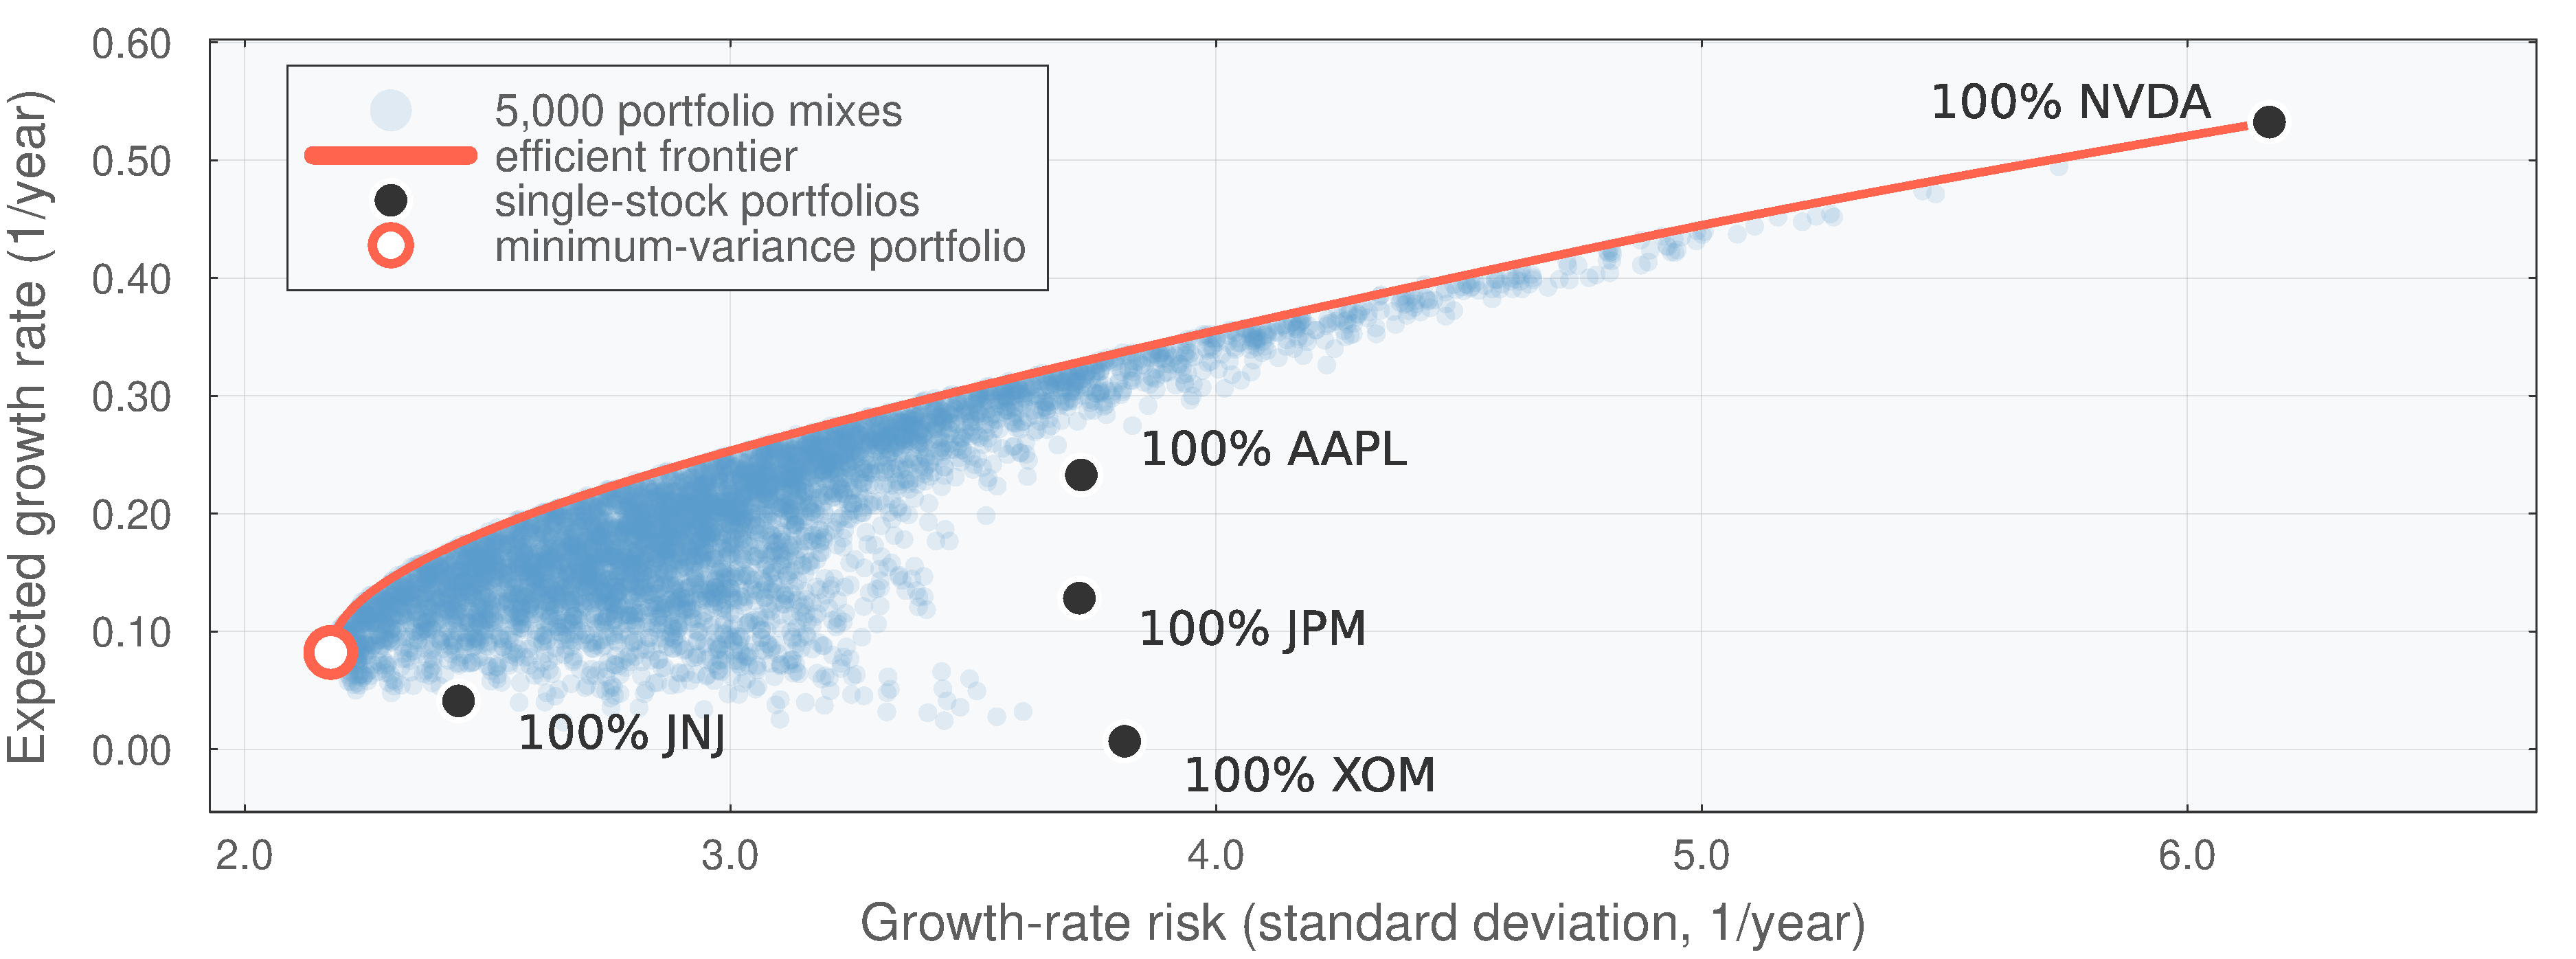
\includegraphics[width=0.98\textwidth,height=0.73\textheight,keepaspectratio]{../figs/Fig-L1a-PortfolioPreview.pdf}
  \end{center}

\end{frame}

\begin{frame}{Options Provide Upside with Limited Downside}
  At the same \$210/\$240 thresholds, the spread requires \$1,508 upfront instead of
  \$22,578. Its loss limit is contractual; a stock stop is not.

  \begin{center}
    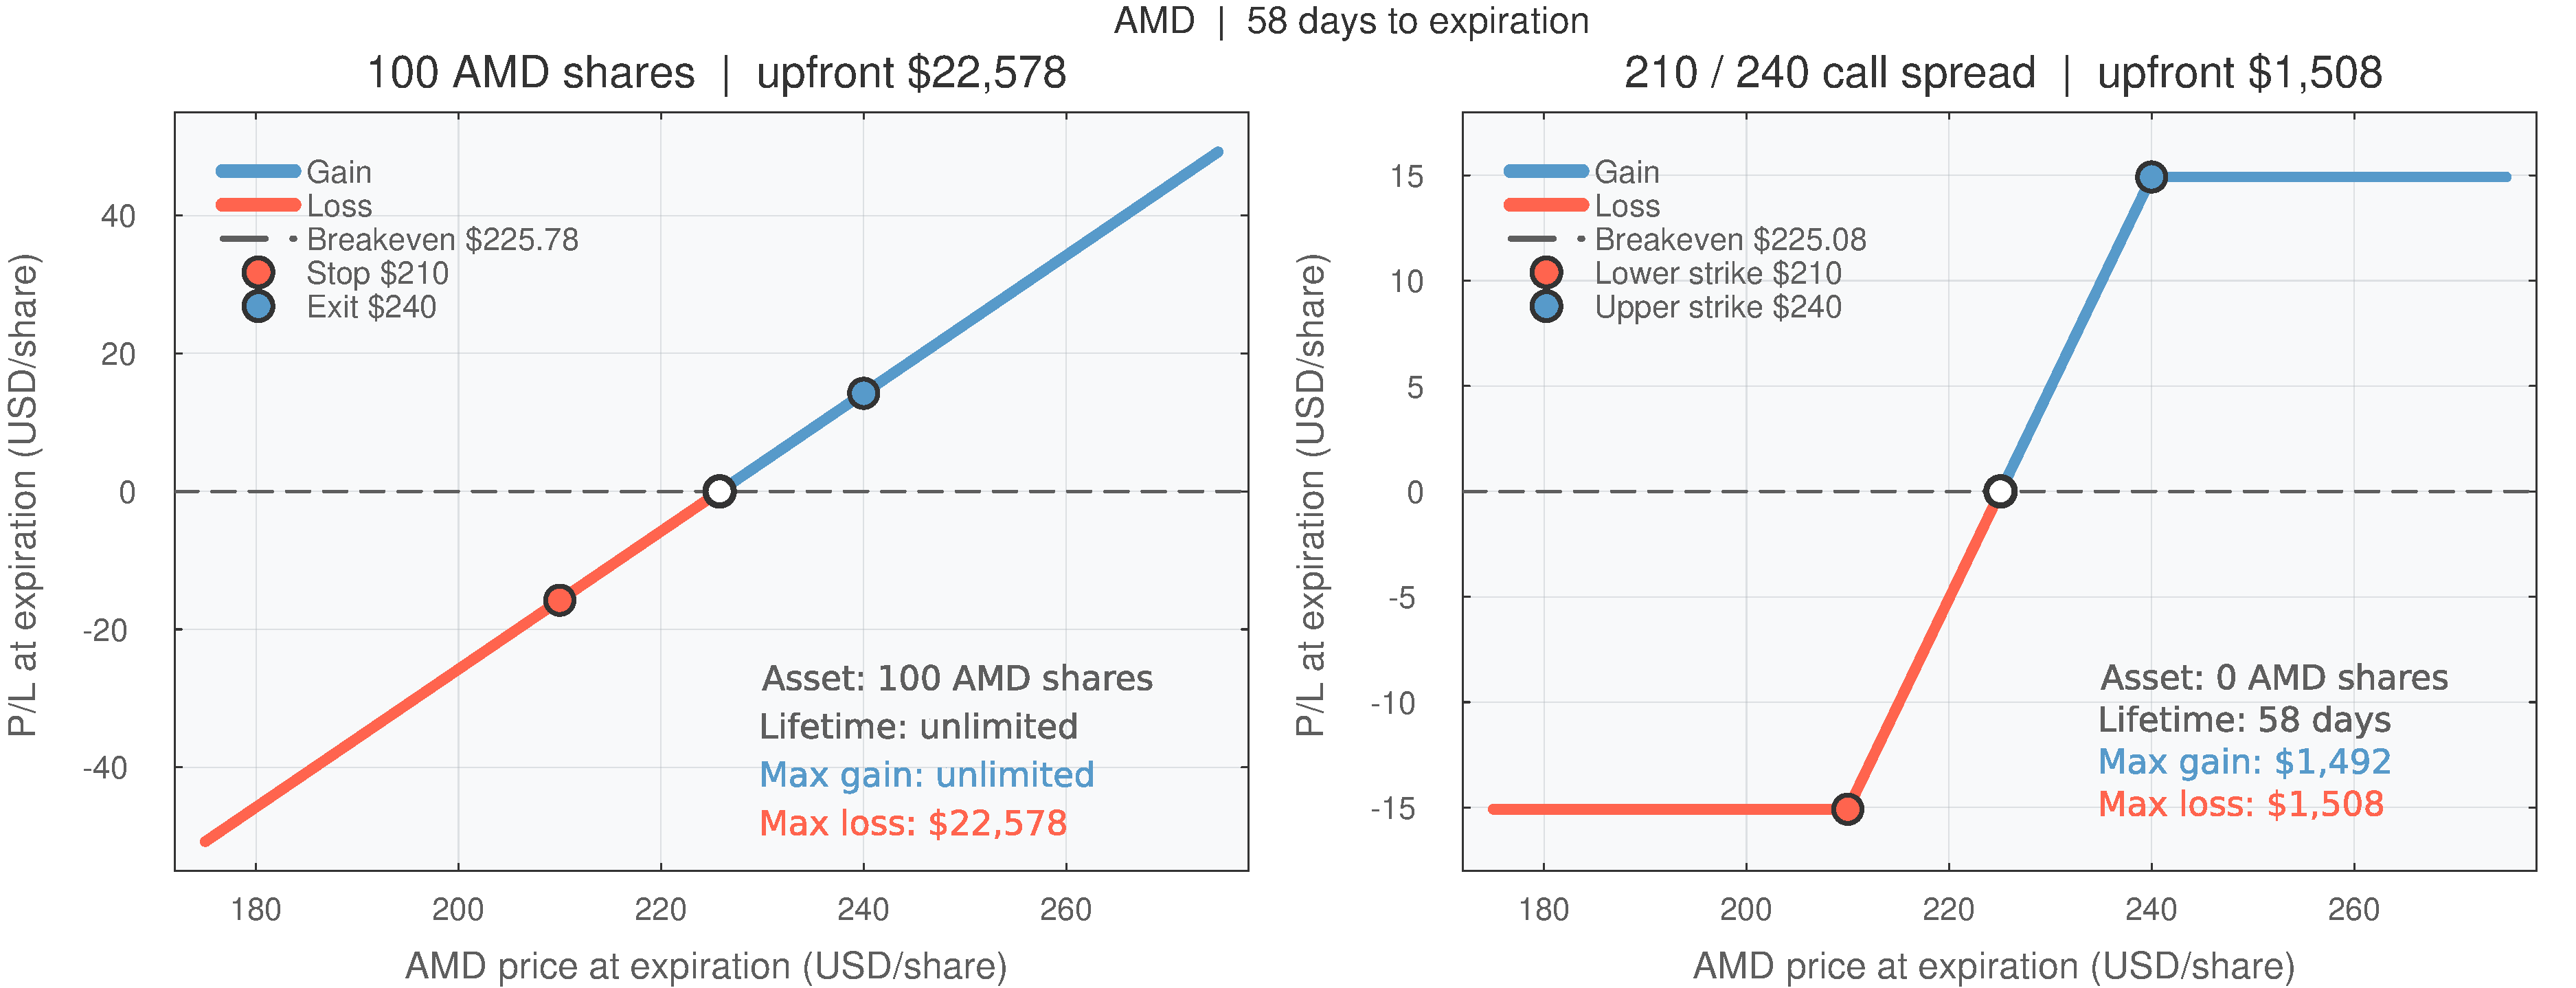
\includegraphics[width=0.98\textwidth,height=0.72\textheight,keepaspectratio]{../figs/Fig-L1a-PayoffPreview.pdf}
  \end{center}

\end{frame}

% ==== federal borrowing and Treasury-market liquidity ====
% Debt to the Penny values are for 2026-08-20. The buyback operation occurred
% on 2026-08-20 and settled on 2026-08-21. Do not update one side without the
% other: the point is the scale comparison on one date. The per-resident figure
% uses the Census projection of 342,620,143 residents on 2026-07-01.
\begin{frame}[t]{Federal Deficits Require Treasury Borrowing}
  \vspace{-0.35em}
  Treasury securities do two jobs: they finance federal deficits and serve as
  the benchmark ``risk-free'' asset in U.S. dollar markets.

  \vspace{0.10em}
  \begin{columns}[T,onlytextwidth]
    \begin{column}{0.43\textwidth}
      \eyebrow{Federal debt | Aug. 20, 2026}

      \vspace{0.15em}
      {\fontsize{34}{36}\selectfont\bfseries\hilite{\$40.03T}\par}
      {\small about \textbf{\hilite{\$117,000 per U.S. resident}}}

      \vspace{0.15em}
      \begin{tabular}{@{}lr@{}}
        \toprule
        {\small Held by the public} & {\small\textbf{\$32.28T}}\\[2pt]
        {\small Intragovernmental}  & {\small\textbf{\$7.75T}}\\[2pt]
        \bottomrule
      \end{tabular}
    \end{column}
    \begin{column}{0.53\textwidth}
      \eyebrow{Liquidity-support buyback | Aug. 20}

      \vspace{0.2em}
      \begin{tabular}{@{}lr@{}}
        \toprule
        {\small Securities offered} & {\small\textbf{\$10.16B}}\\[2pt]
        {\small Announced maximum}  & {\small\textbf{\$4.00B}}\\[2pt]
        {\small Treasury accepted}  & {\small\textbf{\hilite{\$1.86B}}}\\[2pt]
        \bottomrule
      \end{tabular}

      \vspace{0.25em}
      {\small Treasury retired portions of three older issues,
      \hilite{0.006\%} of publicly held debt, to support liquidity.}
    \end{column}
  \end{columns}

  \vspace{0.48em}
  {\large\textbf{Why this matters:}} Treasury yields help set borrowing costs and
  provide the baseline against which other investments are priced.

  % Teaching caveat: ``risk-free'' is the pricing benchmark for promised dollar
  % cash flows, not a claim that Treasury prices cannot fall or that inflation
  % is irrelevant.
  \slidenote{Note:}{Scale comparison, not a bill. Sources: \href{https://fiscaldata.treasury.gov/datasets/debt-to-the-penny/}{Treasury debt}; \href{https://www.treasurydirect.gov/instit/annceresult/press/preanre/2026/BBR_20260820174000.pdf}{buyback}; \href{https://www.census.gov/popclock/}{Census population}.}
\end{frame}

% ==== promises ====
% NO PRODUCT NOUNS ON THIS FRAME. Five cash-flow schedules, nothing else. The
% names arrive on the next frame and that ordering is the entire design: the PBS
% segment later uses the words, so the reveal has to precede the clip.
%
% These five rows RECUR. L1b, L2a, and L2b re-show them verbatim with the same
% numbers, each time answering one more of the open questions. Changing a number
% here means changing it in three later decks.
%
% Amounts are from private/specs/data-l1a/PROMISE-TABLE.md, FRED pull of
% 2026-08-18. Do not edit a number here without re-running that pull.
\begin{frame}{How Should We Compare Future Payments?}
  \vspace{0.1em}
  Suppose five debt instruments each cost \hilite{\$10{,}000} today. Their
  payment schedules differ in \hilite{amount}, \hilite{timing}, and
  \hilite{uncertainty}.

  \vspace{0.35em}
  \begin{center}\small
  {\renewcommand{\arraystretch}{1.0}%
  \begin{tabular}{@{}l@{\hspace{1.2em}}l@{}}
    \toprule
    \textbf{\hilite{A}} & \$10{,}028 back, four weeks from today\\[2pt]
    \textbf{\hilite{B}} & \$236 every six months for 10 years, then \$10{,}000\\[2pt]
    \textbf{\hilite{C}} & \$264 every six months for 30 years, then \$10{,}000\\[2pt]
    \textbf{\hilite{D}} & \$271 every six months for 10 years, then \$10{,}000\\[2pt]
    \textbf{\hilite{E}} & Fixed-rate coupons on inflation-adjusted principal\\
                     & for 10 years, then the adjusted principal\\
    \bottomrule
  \end{tabular}
  }
  \end{center}

  \vspace{0.35em}
  {\centering\large
  \ink{\textbf{Which promise should we choose?}} Let's brainstorm and discuss.\par}

  \slidenote{Rates:}{published rates for 2026-08-18, each scaled to a \$10{,}000 outlay}
\end{frame}


% ==== reveal ====
% Product nouns are allowed from here down, and only from here down.
\begin{frame}{Each Payment Schedule Represents a Different Security}
  \vspace{0.1em}
  \begin{center}\small
  \begin{tabular}{@{}llr@{}}
    \toprule
    & \textbf{\ink{What it is called}} & \textbf{\ink{Market yield}}\\[2pt]
    \midrule
    \textbf{\ink{A}} & 4-week Treasury bill                      & 3.63\%\\
    \textbf{\ink{B}} & 10-year Treasury note                     & 4.71\%\\
    \textbf{\ink{C}} & 30-year Treasury bond                     & 5.28\%\\
    \textbf{\ink{D}} & investment-grade corporate bonds          & 5.42\%\\
    \textbf{\ink{E}} & 10-year inflation-indexed Treasury (TIPS) & 2.41\% \hilite{real}\\[2pt]
    \bottomrule
  \end{tabular}
  \end{center}

  \vspace{0.5em}
  Compare the \hilite{amount}, \hilite{timing}, and \hilite{uncertainty} of the
  payments. The schedule gives the amount and timing. The security type
  identifies which sources of uncertainty matter.

  \slidenote{Careful:}{D is a bond index. E's 2.41\% is a real market yield, not its coupon; TIPS principal adjusts with CPI.}
\end{frame}

% The credit spread here is D minus B -- the corporate index against the
% MATURITY-MATCHED ten-year government row, 5.42 - 4.71 = 71 bp. The design
% spec compared D to C (the 30-year row) and got 11 bp, but D and B are both
% described as ten-year schedules on the previous frame, so a student who
% maturity-matches gets 71 and finds the slide wrong by a factor of five.
% See private/specs/data-l1a/PROMISE-TABLE.md for the full reasoning.
%
% DO NOT swap in the option-adjusted spread series (FRED BAMLC0A0CM, 82 bp).
% It was on this frame briefly and was reverted on 2026-08-20: it is a
% different measure, it was never pulled into data-l1a, and it cannot be
% reproduced from the two rates the previous frame shows. The number on this
% frame must stay the subtraction a student can do from that table.
\begin{frame}{Risk Shapes the Value of Promised Payments}
  \vspace{0.15em}
  Promised cash flows are only the starting point. Their value also depends
  on when we may need the money and which risks we bear.

  \vspace{0.4em}
  \begin{itemize}\setlength{\itemsep}{0.35em}
    \item \hilite{\textbf{C}}\quad\textbf{\ink{Interest-rate risk.}}
      Selling before maturity exposes the investor to market-price changes; when
      yields rise, the bond's price falls.
    \item \hilite{\textbf{D}}\quad\textbf{\ink{Credit and liquidity risk.}}
      The 0.71-percentage-point premium over the ten-year Treasury compensates
      investors for these additional risks.
    \item \hilite{\textbf{E}}\quad\textbf{\ink{Inflation protection.}}
      Because TIPS principal adjusts with CPI, its 2.41\% real yield measures
      purchasing-power growth rather than nominal dollars.
  \end{itemize}

  \vspace{0.35em}
  \ink{A sound comparison considers both the payments and the risks that
  determine their value.}
\end{frame}

% ==== svb ====
% The clip plays IN FULL. This frame states the causal chain that students
% should watch for: withdrawals created a cash need, forcing SVB to sell
% long-term securities after higher rates had reduced their market value.
\begin{frame}{Silicon Valley Bank (SVB) Needed Cash to Cover Withdrawals}
  \vspace{0.35em}
  \begin{columns}[T,onlytextwidth]
    \begin{column}{0.27\textwidth}
      {\fontsize{30}{32}\selectfont\vnmedium\hilite{\$200B}\par}
      {\small assets in March 2023}
    \end{column}
    \begin{column}{0.69\textwidth}
      Depositors became concerned and began withdrawing money.

      \vspace{0.55em}
      SVB needed cash, so it sold long-term securities before maturity.
    \end{column}
  \end{columns}

  \vspace{0.9em}
  Interest rates had risen, so those securities were worth less than SVB had
  paid.

  \vspace{0.75em}
  {\large\vnmedium\ink{Interest-rate risk became a liquidity problem.}}

  \slidenote{Clip:}{\href{\svburl}{PBS NewsHour, 28 March 2023, 6 minutes}}
\end{frame}

% ==== summary ====
% Summary frames carry all three parts: one summary sentence, exactly three
% key takeaways, one concluding sentence. See vnslides.sty rule 7.
\begin{frame}[t]{Summary}
  Today we established why the course matters and introduced our first
  investment decision.

  \vspace{0.45em}
  \decklabel{Key takeaways}
  \vspace{0.2em}
  \begin{itemize}\setlength{\itemsep}{0.35em}
    \item \textbf{\ink{The course moves from assets to decisions.}}
      We value debt, equity, and derivatives, then combine and test them in
      financial strategies.
    \item \textbf{\ink{Markets connect savings to investment.}}
      Households, Cornell, companies, and the Treasury use markets to save,
      invest, raise funds, or finance deficits.
    \item \textbf{\ink{A payment schedule is only the starting point.}}
      Amount, timing, interest-rate, credit, liquidity, and inflation risk all
      affect an investment's value.
  \end{itemize}

  \vspace{0.45em}
  Next, we build our first comparison rule: use the time value of money to
  compare payments made on different dates.
\end{frame}

% ==== reading ====
% The four links from the deleted L1a reading list. Offered, not assigned: there
% is no notes packet to hold anyone to, and L1b teaches this material properly.
% All four verified HTTP 200 on 2026-08-19.
\begin{frame}{Further Reading}
  \vspace{0.4em}
  These readings are optional and will not appear on a problem set. Use them if
  you want more background on the Federal Reserve, monetary policy, or the
  Treasury.

  \vspace{0.9em}
  \begin{itemize}\setlength{\itemsep}{0.55em}
    \item \href{https://www.federalreserve.gov/aboutthefed/structure-federal-reserve-system.htm}{\emph{The Structure and Functions of the Federal Reserve System}}, Federal Reserve Board: who does what inside the Federal Reserve.
    \item \href{https://www.federalreserve.gov/economy-at-a-glance-policy-rate.htm}{\emph{Economy at a Glance: Policy Rate}}, Federal Reserve Board: how the Fed reports and carries out interest-rate policy.
    \item \href{https://www.newyorkfed.org/aboutthefed/fedpoint/fed01.html}{\emph{Fedpoints: Federal Reserve System}}, Federal Reserve Bank of New York: a short overview of how the system is organized.
    \item \href{https://home.treasury.gov/about/general-information/role-of-the-treasury}{\emph{Role of the Treasury}}, U.S. Department of the Treasury: what the Treasury does and how it differs from the Federal Reserve.
  \end{itemize}
\end{frame}


\end{document}
